\documentclass[a4paper, 12pt, addpoints]{exam}
\usepackage{IfbaListas}
%==============================================================
\NumList{1} %NÚMERO DA LISTA
\Assunto{Limite \& Continuidade}
%==============================================================
%=========================================================
%------------Cabeçalho e rodapé 
%=========================================================
\pagestyle{headandfoot}%{head}%empty
\firstpageheader{}{}{}
\runningheader{\disciplina}{}{Lista \numlist: \assunto}
\runningheadrule
\firstpagefooter{\copyright \professor}{}{Pag. \thepage\ de \numpages}
\runningfooter{\iflastpage{Outros templates em \href{http://gg.gg/profwaldexsantos}{gg.gg/profwaldexsantos}}{\copyright Valdex Santos}}{}{Pag. \thepage\ de \numpages}
\runningfootrule
%===============================================================
%INFORMAÇÕES SOBRE A AVALIAÇÃO
\nomeInst{Instituto Federal da Bahia}
\logoInst{
\includegraphics[scale=0.17]{Figs/ifbajequie.jpg}}
\Campus{Jequié} %PARA ENSINO FUNDAMENTAL OU MÉDIO-COMENTE ESTA LINHA COM %
\nomeCurso{nome do curso} %Se não for curso superior, basta comentar esta linha ou deixar em branco
\nomeDisciplina{Cálculo Diferencial e Integral I}
\Semestre{}
\nomeProfessor{Nome do Professor}
\Aluno{}
\matriculaAluno{}
%===============================================================
 %CARREGA AS INFORMAÇÕES GERAIS DO PROFESSOR, ESCOLA ETC
%==============================================================

%COMEÇO DO DOCUMENTO
\begin{document}
\info\vspace{-1 cm} %Imprime as informações do cabeçalho programada no pacote 
% inicia a gravacao da resposta no arquivo "ans" cujo nome externo é gabarito 
\Opensolutionfile{ans}[Gabarito] 
%*****************************************************************************
\begin{questions}%COMEÇA O AMBIENTE DE QUESTÕES
\question Calcule os limites abaixo:
\begin{multicols}{3}
\begin{enumerate}[a)]
\item  $\lim _{x \rightarrow-2} \frac{4-x^{2}}{2+x}$
\item $\lim _{x \rightarrow 3} \frac{x^{2}-4 x+3}{x^{2}-x-6}$
\item $\lim _{x \rightarrow 1} \frac{x^{3}-1}{5 x-5}$
\item $\lim _{x \rightarrow-2} \frac{8+x^{3}}{4-x^{2}}$
\item $\lim _{x \rightarrow 2} \frac{x^{4}-16}{8-x^{3}}$
\item $\lim _{x \rightarrow 1} \frac{\sqrt{x}-1}{x-1}$
\item $\lim _{x \rightarrow-1} \frac{1-x^{2}}{x+\sqrt{2+x}}$
\item $\lim _{x \rightarrow 7} \frac{2-\sqrt{x-3}}{x^{2}-49}$
\item $\lim _{x \rightarrow 4} \frac{3-\sqrt{5+x}}{1-\sqrt{5-x}}$
\end{enumerate}
\end{multicols}
\begin{resp}~
\begin{multicols}{5}
\begin{enumerate}[a)]
\item 4
\item 2/5
\item 3/5
\item 3
\item -8/3
\item 1/2
\item 4/3
\item -1/56
\item -1/3
\end{enumerate}
\end{multicols}
\end{resp}
\question  Calcule os limites utilizando o \textit{``Limite Fundamental Exponencial''}:
\begin{multicols}{3}
\begin{enumerate}[a)]
\item $\lim _{x \rightarrow 0}(1+2 x)^{1 / x}$
\item $\lim _{x \rightarrow 0} \frac{3^{x}-1}{x}$
\item $\lim _{x \rightarrow 0} \frac{e^{x}-1}{4 x}$
\end{enumerate}
\end{multicols}
\begin{resp}
\begin{multicols}{3}
\begin{enumerate}[a)]
\item $e^2$
\item $\ln(3)$
\item $1/4$
\end{enumerate}
\end{multicols}
\end{resp}
\question  Calcule os limites utilizando o \textit{``Limite Fundamental Trigonométrico''}:
\begin{multicols}{4}
\begin{enumerate}[a)]
\item $\lim _{x \rightarrow 0} \frac{\operatorname{sen}(2 x)}{x}$
\item $\lim _{x \rightarrow 0} \frac{\operatorname{sen}(5 x)}{\operatorname{sen}(3 x)}$
\item $\lim _{x \rightarrow 0} \frac{\cos (x)-1}{x}$
\item $\lim _{x \rightarrow 0} \frac{\operatorname{tg}(x)}{x}$
\end{enumerate}
\end{multicols}
\begin{resp}
\begin{multicols}{4}
\begin{enumerate}[a)]
\item 2
\item 5/3
\item 0
\item 1
\end{enumerate}
\end{multicols}
\end{resp}
\question Determine, se possível, as constantes $a$ e $b \in \mathbb{R}$ de modo que as funções abaixo sejam contínuas no ponto $x_{o}$, sendo:
\begin{multicols}{2}
\begin{enumerate}[a)]
\item $f(x)=\left\{\begin{array}{l}3 a x^{2}+2, x<1 \\ x-2, x \geq 1\end{array}\left(x_{o}=1\right)\right.$
\item $g(x)=\left\{\begin{array}{l}a x^{2}+2, x \neq 1 \\ a^{2}, x=1\end{array}\left(x_{o}=1\right)\right.$
\item $f(x)=\left\{\begin{array}{l}3 x-3, x>-3 \\ a x, x=-3 \\ b x^{2}+1, x<-3\end{array}\left(x_{o}=-3\right)\right.$
\item $g(x)=\left\{\begin{array}{l}2 a \cdot \cos (\pi+x)+1, x<0 \\ 7 x-3 a, x=0 \\ b-2 x^{2}, x>0\end{array} \quad\left(x_{o}=0\right)\right.$
\end{enumerate}
\end{multicols}
\begin{resp}~
\begin{multicols}{2}
\begin{enumerate}[a)]
\item $a=-1$
\item $a=-1$ ou $a=2$
\item $a=4$ e $b=-13/9$
\item $a=-1$ e $b=3$
\end{enumerate}
\end{multicols}
\end{resp}
\question (\textbf{Problema do circuito RL em série})
No circuito da Fig. \ref{Fig:Circ} abaixo, temos uma associação em série de um resistor (símbolo $R$) e um indutor (símbolo $L$). Da segunda lei de Kirchhoff (lei das voltagens) e do estudo das equações diferenciais, pode-se mostrar que a corrente $i$ no circuito é dada por
\begin{equation}
  i(t)=\dfrac{E}{R}+ce^{-\left(\frac{R}{L}\right)t}\label{eq.resistor}
\end{equation}
onde $E$ é uma bateria de voltagem fixa, $c$ é uma constante real e $t$ é o tempo.
\begin{figure}[hbt]
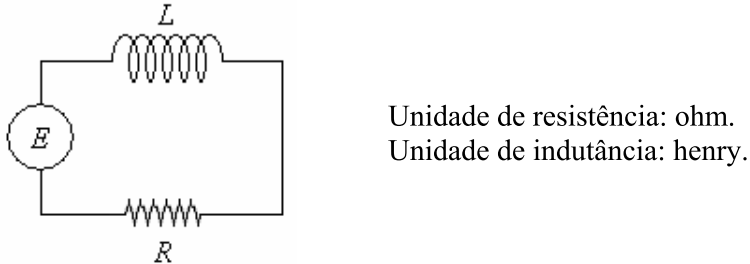
\includegraphics[scale=0.65]{Figs/L1/Resistor.png}\label{fig-resistorL1}
\caption{Representação de um circuito}
\label{Fig:Circ}
\end{figure}\\
\textbf{Exercício 1:} Se uma bateria de 12 volts é conectada a um circuito em série (como na figura acima) no qual o indutor é de 1/2 henry e o resistor é de 10 ohms, determine o valor da constante $c$ e a corrente $i(t)$. Considere a corrente inicial e o tempo inicial iguais a zero.\\
\textbf{Exercício 2:} Determine $\displaystyle\lim_{t\to \infty} i(t)$, sendo $i(t)$ da equação (\ref{eq.resistor})\\
\textbf{Exercício 3-Observações:} 
\begin{enumerate}[a)]
\item O que acontece com o termo $ce^{-\left(\frac{R}{L}\right)t}$ quanto $\displaystyle {t\to \infty}$? \textbf{Explique!} Tal termo é usualmente denominado \textbf{corrente transitória}. \textbf{Explique!}
\item A razão $E/R$ é chamada \textbf{corrente estacionária}. \textbf{Explique!} 
\item Após um longo período, a corrente no circuito é governada praticamente pela lei de Ohm $E= Ri $. \textbf{Explique!}
\end{enumerate}
\begin{resp}
 -
\end{resp}
\end{questions}

\vspace{1cm}
\begin{center}
    \section*{Gabarito}
\end{center}
\Closesolutionfile{ans}% finaliza a gravação das respostas
\input{Gabarito} %imprime as soluções
\end{document}